\documentclass{standalone}
\usepackage{tkz-base}
\usepackage{tkz-fct}
\usepackage{tkz-euclide}
\usepackage{tikz}
\begin{document}
    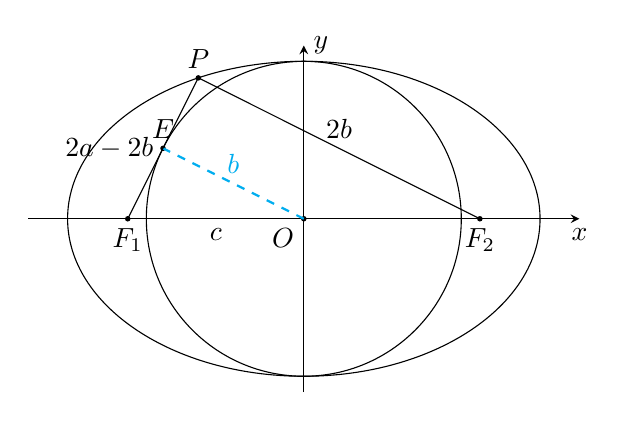
\begin{tikzpicture}
        \pgfmathsetmacro\x{3.5}
        \pgfmathsetmacro\y{2.2}
        \pgfmathsetmacro\a{3}
        \pgfmathsetmacro\b{2}
        \pgfmathsetmacro\c{sqrt(abs(\a^2-\b^2))}
        \pgfmathsetmacro\px{-1.34}
        \pgfmathsetmacro\py{sqrt((\b^2)*(1-((\px)^2)/(\a^2)))}
        \coordinate (O) at (0,0);
        \coordinate (F1) at (-\c,0);
        \coordinate (F2) at (\c,0);
        \coordinate (P) at (\px,\py);
        \coordinate (E) at ($(P)!0.5!(F1)$);
        \draw[-stealth] (-\x,0) -- (\x,0) node [below] {$x$};
        \draw[-stealth] (0,-\y) -- (0,\y) node [right] {$y$};
        \fill (O) node [below left] {$O$} circle (1pt);
        \fill (F1) node [below] {$F_1$} circle (1pt);
        \fill (F2) node [below] {$F_2$} circle (1pt);
        \fill (P) node [above] {$P$} circle (1pt);
        \fill (E) node [above] {$E$} circle (1pt);
        \draw (F1) -- (P)node [pos=0.5,left] {$2a-2b$} -- (F2)node [pos=0.5,above] {$2b$};
        \draw[cyan,dashed,thick] (O) -- (E) node [pos=0.5,above] {$b$};
        \path (O) -- (F1) node [pos=0.5,below] {$c$} ;
        \draw (O) circle [x radius=\a,y radius=\b];
        \draw (O) circle (\b);

    \end{tikzpicture}
\end{document}